
\chapter{基本事項}

\section{正規分布}

\section{基礎知識}

実験の測定値($x_1,x_2,...,x_n$)は、真の値$X$の周りにふらつきを持って得られる。
究極的な目標は実験の精度を極限にまで高めて、真の値$X$を知ることである。

\subsubsection{平均 $\bar{x}$}
$n$点測定した結果を評価する時によく用いられるのが平均(算術平均or相加平均)である。

\begin{equation}
  \bar{x} = \frac{x_1 + x_2 + ... + x_n}{n}  = \frac{1}{n} \sum_{i=1}^{n} x_i
\end{equation}


\subsubsection{分散 $V$}
測定値がどれくらいばらついている(分散している)かの指標。平均値の周りにピッタリ分布していれば、
分散は小さくなり、平均値から大きかったり小さかったりすると、分散は大きくなる。

\begin{equation}
  V= \frac{1}{n}\sum_{i=1}^{n} (x_{i}-\bar{x})^{2} = \int (x-\bar{x})^2f(x)dx
\end{equation}

\subsubsection{偏差 $\sigma$}
分散の平方根を取ったもの
\begin{equation}
  \sigma = \sqrt{V}
\end{equation}

\subsubsection{期待値}
ある確率変数$X$に対する期待値は、$E[X]$と表される。 確率によって重み付けして平均を計算したもので、

\begin{equation}
  E[x] = \frac{p_1\times x_1+ p_2\times x_2+...+ p_n \times x_n}{n} = \frac{1}{n}\sum_{i=1}^{n} p_ix_i
\end{equation}

重要な性質として、実験結果$x=(x_1,x_2,...,x_n)$の期待値は、

\begin{equation}
  E[x] = \lim_{n\to\infty} = \frac{1}{n}\sum_{i=1}^{n} p_ix_i = \frac{1}{n}\sum_{i=1}^{n} p_ix_i
\end{equation}



\subsubsection{母集団と標本}
ある母集団から確率変数$X$を予想する場合。無限個のサンプル取得が可能であれば、 $X$の平均値(=期待値)は

\begin{equation}
  \mu = \bar{X} = \lim_{n\to\infty} \left(\frac{1}{n} \sum_{i=1}^{n} x_i \right)
\end{equation}

母平均の期待値 $E[\mu]$は、
\begin{equation}
  E[\mu] = \lim_{n\to\infty}\sum_{i=1}^{n}
\end{equation}

で表される。母集団から無限個のサンプルを取得すれば、真の値(母平均)を計算することができることを意味する。
また、母集団の分散(母分散)は

\begin{equation}
  V= \frac{1}{n}\sum_{i=1}^{n} (x_{i}-\mu)^{2}
\end{equation}

で表される。

実際には$n$の値は有限であり、母平均$\mu$や母分散$V$を計算することはできない。
ここで注意が必要である。
\subsubsection{標本分散}
\begin{equation}
  E((X-\bar{X})^2) = \sum_{i=1}^{n} (X_i - \bar{X})^2 = \sum_{i=1}^{n} \left(X_i - \frac{1}{n}\sum_{j=1}^{n} X_j \right)^2
  =
\end{equation}

% ====================================
\section{確率分布}
\subsubsection{ポワソン分布}
\label{subsubsec:poisson}
平均 $\lambda$ 回発生する確率事象が、$x$ 回起こる確率

\begin{table}[h]
  \centering
  \begin{tabular}{lll}
    確率密度関数 & $f(x)=\frac{e^{\lambda}~\lambda^{x}}{x!}$   \\
    期待値      & $E(x)=\lambda$    \\
    分散        & $V(x)=\lambda$
  \end{tabular}
\end{table}

事象が起こる平均値$\lambda$が大きくなるほど、形がガウス分布に近づいていく。
十分に大きくなると$\mu=\lambda$、$V=\lambda$のガウス分布として近似できる。

\begin{figure}[h]
  \centering
  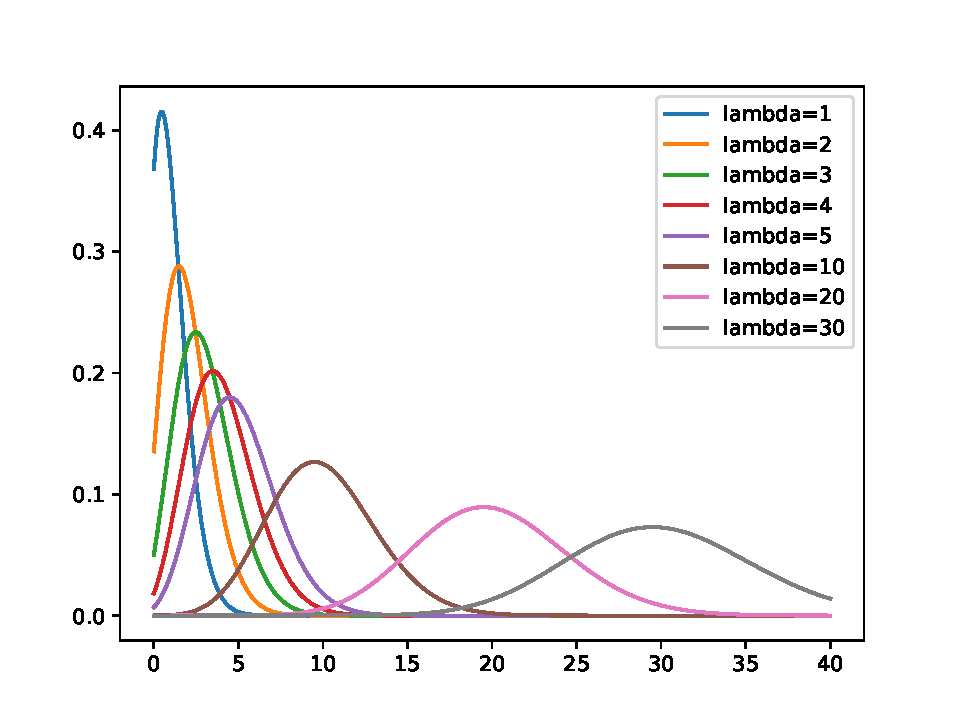
\includegraphics[scale=0.5]{python/poisson_scan.pdf}
  \caption{異なる平均値を取ったときのポワソン分布。平均$\lambda$が大きくなるほど、ガウス分布のような形状になっていくのが分かる。}
\end{figure}

\subsubsection{正規分布(ガウス分布)}

\begin{table}[h]
  \centering
  \begin{tabular}{lll}
    確率密度関数 & $f(x)=\frac{1}{\sqrt{2\pi} \sigma}e^{-\left(\frac{(x-\mu)^2}{2\sigma^2}\right)}$   \\
    期待値      & $E(x)=\mu$    \\
    分散        & $V(x)=\sigma$
  \end{tabular}
\end{table}

\begin{itembox}[l]{ガウス分布の性質その1}
  確率変数$X$が$N(\mu,\sigma^2)$の正規分布に従うなら、$aX+b$は$N(a\mu+b,a^2\sigma^2)$の正規分布に従う
\end{itembox}




\section{誤差論}
\subsubsection{誤差の伝播}
N点の計測($x_1, x_2, ..., x_n$)を行う。測定値それぞれに誤差がついている場合($x_1\pm\Delta x_1, x_2\pm\Delta x_2, ..., x_n\pm\Delta x_n$)、測定結果の合計、平均にはどのような誤差が付くか。

\subsubsection{合計の誤差}

\begin{equation}
  y=\Sigma_i~x_i=x_1+x_2+...+x_n=n\times\frac{1}{n}(x_1+x_2+...+x_n)=n\bar{x}
\end{equation}

誤差の和はyに対して、

\begin{equation}
  \Delta y = \sqrt{\left(\frac{\partial}{\partial x_1}y \right)^2 \Delta x_1^2 + ... + } = \sqrt{\Sigma_{i=1}\left(\frac{dy}{dx_i}\right)^2\Delta x_i^2}
\end{equation}

として伝搬する(誤差伝搬の公式).
今の場合、
\begin{equation}
  \frac{\partial}{\partial x_1}n\times \frac{1}{n}(x_1+x_2+...+x_n)=1
\end{equation}

となるので、

\begin{equation}
  \Delta y=\sqrt(\Sigma(\Delta x_i)^2)
\end{equation}

測定値$x_{i}$の分散は、測定したn点から事前に計算される。
なので誤差の伝播の式を進めると、
\begin{equation}
  \Delta y=\sqrt{ns^2}=\sqrt{n}s
\end{equation}
となる。

\subsubsection{平均の誤差}
測定値の平均値には、
\begin{equation}
  \bar{x}=\frac{1}{n}\Sigma x_i
\end{equation}

誤差伝搬の式を適用して、
\begin{equation}
  \Delta \bar{x} = \sqrt{n\times\left(\frac{1}{n}\right)^2s^2}=\frac{1}{\sqrt{n}}
\end{equation}

この式は、平均値の誤差は測定点の数のルートN倍で小さくなっていくことを示している。測定を繰り返し行い、平均を得た場合にどのように誤差が小さくなっていくかを示している。

- 計数の誤差
- 計数$N$の統計誤差は$\sqrt{N}$で表される

\subsubsection{ヒストグラムにおける誤差}
ここまでの議論は、例えば粒子の不変質量を測定した場合に、あるイベントでは$m_1$[GeV]、あるイベントでは$m_2$[GeV]、...と測定した時に、その測定量に対してどれくらい誤差が付いているかを論じてきた。
議論をもう一度繰り返すと、$n$回測定した質量の平均値は、

\begin{equation}
  \bar{m}=\frac{1}{n}\Sigma m_i
\end{equation}

測定結果の分散は、

\begin{equation}
  V=\Sigma(m_i-\bar{\mu})・・・(☆)
\end{equation}

で表される。しかし、これらの議論はヒストグラムの場合には少し特殊な議論となる。よく不変質量の分布をヒストグラムにしたりして議論を進めていくが、この時によく「ヒストグラムにエラーバーを付けて」と言われるが、このエラーバーはここまでの誤差とは若干違っている。(☆)の誤差は不変質量の測定値に付くものであって、ヒストグラムのそれぞれのビンにつくものではない。

\subsection{ビンにつく誤差}
「ヒストグラムのエラー」は、そのビンにいる統計数に対して考える。よくみるヒッグス粒子の不変質量を例に取ってみよう。(☆)の議論はヒッグス質量125GeVに対して$125GeV \pm \sigma_{H}$ という形で付くものである。これは強いて言うなら下図の横方向(x軸方向)に対しての誤差である、

では、図に示されている縦方向の誤差は一体なんでしょうか?これこそが高エネ実験領域でよく耳にする「統計誤差」というものである。

\subsubsection{考え方}
例えば1番目のビンに注目する。このビンでカウントされている事象数を仮に460事象と読み取ることにする。
これを「とある確率分布に従う事象を観測し、平均値460事象観測した」と捉える。よく用いられる確率分布はポワソン分布である(\ref{subsubsec:poisson}節)。
簡単に分散$V=460$、$\sigma=\sqrt{460}$と求めることができる。これがヒストグラムの計量の際の誤差である。感覚的には、縦方向に(各ビンに)ある確率分布があって、それらの平均値をつなぐようにしてヒッグス質量分布が計算されているとすればいい。

\subsubsection{誤差はどうなっていくか}
統計量が溜まってくると、1ビン〜10000事象とかがあるかもしれない。こういうときにポワソン分布でヒストグラムのエラーバーを考えていいのか?という疑問が湧いてくる。答えは**ガウス分布**を使う、が、「考え方」は変わらないということである。

- 二項分布→ポワソン分布
- 二項分布において$\lambda$を一定にして、$n$を大きく、$p$を小さくするとポワソン分布になる
- ポワソン分布→ガウス分布
- ポワソン分布で$\lambda$を大きくすると、期待値$\lambda$、分散$\lambda$のガウス分布になる
- 二項分布→ガウス分布
- 期待値$np$、分散$np(1-p)$の両方が大きい場合、期待値$np$、$分散np(1-p)$のガウス分布になる

上記の関係性を思い出せば、1ビンあたりの統計量(=1ビンで観測したイベントの期待数)が大きくなっても、結局は分散$\lambda$のガウス分布に従っているので、ヒストグラムのエラーバーはやはり$\sqrt{N}$になる。

つまりヒストグラムのエラーバーは、

$N\pm\sqrt{N}$

の関係で成り立っている(ポワソン分布orガウス分布に由来するものであることに留意)。


\subsection{「誤差は$\frac{1}{\sqrt{N}}$で小さくなっていく」の真実}
誤差の大きさそのものが$\frac{1}{\sqrt{N}}$なのではなく、ここで言っている誤差は「XX\%」の誤差に相当するものである。ヒストグラムの誤差は、

\begin{equation}
  N\pm\sqrt{N}
\end{equation}

で付くものだったから、1ビンに対する誤差は

\begin{equation}
  \frac{\sqrt{N}}{N}\times 100 = \frac{1}{\sqrt{N}} \%
\end{equation}

である。つまり、1ビンに入る統計数が多くなればなるほど、統計量が増えれば増えるほど、誤差は、$\frac{1}{\sqrt{N}}$で小さくなっていきます。
なので、できる限り統計量を貯める、という至極まっとうな感想が生まれてきます。

ちなみに、例えばあるビンの統計数が1事象だった場合の誤差は、

\begin{equation}
  1\pm 1
\end{equation}

で、「なんだ、誤差の大きさは1じゃん、小さいじゃん」と思うかもしれないが、

\begin{equation}
  \frac{\sqrt{1}}{1}\times 100 = 100 \%
\end{equation}

の誤差が付いているという事実を忘れてはならない。ちなみに100事象貯めれば、

\begin{equation}
  \frac{\sqrt{100}}{100}\times 100 = 10 \%
\end{equation}

10\%の誤差にまで削減することができるのである。

\section{共分散}

\section{モーメント}
確率密度関数$f(x)$に対して、$x^n$の期待値を定義することができる($n$は整数)。
それらはモーメントと呼ばれ:
\begin{equation}
  a_n \coloneqq E[x_n]
\end{equation}
と定義される。
\begin{itemize}
  \item $a_1$:平均値(mean)
\end{itemize}

また、$x$が平均値からどれだけ離れているか(散らばっているか)を表す量として中央モーメント
\begin{equation}
  m_n \coloneqq E[(x-\mu)^n]
\end{equation}
が定義されている。
$n=2$は分散として知られている値であり、
\begin{equation}
  m_2 = E[(x-\mu)^2] = \sigma^2 = V[x]
\end{equation}


\section{共分散の定義}

確率密度関数$f(x,y)$の場合、同様に$x$、$y$に対するモーメントも定義できるが、それらの相関も計算することができ(共分散; covariance)
\begin{equation}
  \rm{cov}[x,y] \coloneqq E[xy] - E[x]E[y]
\end{equation}
さらに、相関(correlation)も計算することができ、
\begin{equation}
  \rho \coloneqq \frac{\rm{cov}[x,y]}{\sigma_x\sigma_y}
\end{equation}
これらは多次元への拡張も可能である。
